\documentclass[]{article}
\usepackage{lmodern}
\usepackage{amssymb,amsmath}
\usepackage{ifxetex,ifluatex}
\usepackage{fixltx2e} % provides \textsubscript
\ifnum 0\ifxetex 1\fi\ifluatex 1\fi=0 % if pdftex
  \usepackage[T1]{fontenc}
  \usepackage[utf8]{inputenc}
\else % if luatex or xelatex
  \ifxetex
    \usepackage{mathspec}
  \else
    \usepackage{fontspec}
  \fi
  \defaultfontfeatures{Ligatures=TeX,Scale=MatchLowercase}
\fi
% use upquote if available, for straight quotes in verbatim environments
\IfFileExists{upquote.sty}{\usepackage{upquote}}{}
% use microtype if available
\IfFileExists{microtype.sty}{%
\usepackage{microtype}
\UseMicrotypeSet[protrusion]{basicmath} % disable protrusion for tt fonts
}{}
\usepackage[margin=1in]{geometry}
\usepackage{hyperref}
\hypersetup{unicode=true,
            pdftitle={Regresion},
            pdfborder={0 0 0},
            breaklinks=true}
\urlstyle{same}  % don't use monospace font for urls
\usepackage{color}
\usepackage{fancyvrb}
\newcommand{\VerbBar}{|}
\newcommand{\VERB}{\Verb[commandchars=\\\{\}]}
\DefineVerbatimEnvironment{Highlighting}{Verbatim}{commandchars=\\\{\}}
% Add ',fontsize=\small' for more characters per line
\usepackage{framed}
\definecolor{shadecolor}{RGB}{248,248,248}
\newenvironment{Shaded}{\begin{snugshade}}{\end{snugshade}}
\newcommand{\AlertTok}[1]{\textcolor[rgb]{0.94,0.16,0.16}{#1}}
\newcommand{\AnnotationTok}[1]{\textcolor[rgb]{0.56,0.35,0.01}{\textbf{\textit{#1}}}}
\newcommand{\AttributeTok}[1]{\textcolor[rgb]{0.77,0.63,0.00}{#1}}
\newcommand{\BaseNTok}[1]{\textcolor[rgb]{0.00,0.00,0.81}{#1}}
\newcommand{\BuiltInTok}[1]{#1}
\newcommand{\CharTok}[1]{\textcolor[rgb]{0.31,0.60,0.02}{#1}}
\newcommand{\CommentTok}[1]{\textcolor[rgb]{0.56,0.35,0.01}{\textit{#1}}}
\newcommand{\CommentVarTok}[1]{\textcolor[rgb]{0.56,0.35,0.01}{\textbf{\textit{#1}}}}
\newcommand{\ConstantTok}[1]{\textcolor[rgb]{0.00,0.00,0.00}{#1}}
\newcommand{\ControlFlowTok}[1]{\textcolor[rgb]{0.13,0.29,0.53}{\textbf{#1}}}
\newcommand{\DataTypeTok}[1]{\textcolor[rgb]{0.13,0.29,0.53}{#1}}
\newcommand{\DecValTok}[1]{\textcolor[rgb]{0.00,0.00,0.81}{#1}}
\newcommand{\DocumentationTok}[1]{\textcolor[rgb]{0.56,0.35,0.01}{\textbf{\textit{#1}}}}
\newcommand{\ErrorTok}[1]{\textcolor[rgb]{0.64,0.00,0.00}{\textbf{#1}}}
\newcommand{\ExtensionTok}[1]{#1}
\newcommand{\FloatTok}[1]{\textcolor[rgb]{0.00,0.00,0.81}{#1}}
\newcommand{\FunctionTok}[1]{\textcolor[rgb]{0.00,0.00,0.00}{#1}}
\newcommand{\ImportTok}[1]{#1}
\newcommand{\InformationTok}[1]{\textcolor[rgb]{0.56,0.35,0.01}{\textbf{\textit{#1}}}}
\newcommand{\KeywordTok}[1]{\textcolor[rgb]{0.13,0.29,0.53}{\textbf{#1}}}
\newcommand{\NormalTok}[1]{#1}
\newcommand{\OperatorTok}[1]{\textcolor[rgb]{0.81,0.36,0.00}{\textbf{#1}}}
\newcommand{\OtherTok}[1]{\textcolor[rgb]{0.56,0.35,0.01}{#1}}
\newcommand{\PreprocessorTok}[1]{\textcolor[rgb]{0.56,0.35,0.01}{\textit{#1}}}
\newcommand{\RegionMarkerTok}[1]{#1}
\newcommand{\SpecialCharTok}[1]{\textcolor[rgb]{0.00,0.00,0.00}{#1}}
\newcommand{\SpecialStringTok}[1]{\textcolor[rgb]{0.31,0.60,0.02}{#1}}
\newcommand{\StringTok}[1]{\textcolor[rgb]{0.31,0.60,0.02}{#1}}
\newcommand{\VariableTok}[1]{\textcolor[rgb]{0.00,0.00,0.00}{#1}}
\newcommand{\VerbatimStringTok}[1]{\textcolor[rgb]{0.31,0.60,0.02}{#1}}
\newcommand{\WarningTok}[1]{\textcolor[rgb]{0.56,0.35,0.01}{\textbf{\textit{#1}}}}
\usepackage{graphicx,grffile}
\makeatletter
\def\maxwidth{\ifdim\Gin@nat@width>\linewidth\linewidth\else\Gin@nat@width\fi}
\def\maxheight{\ifdim\Gin@nat@height>\textheight\textheight\else\Gin@nat@height\fi}
\makeatother
% Scale images if necessary, so that they will not overflow the page
% margins by default, and it is still possible to overwrite the defaults
% using explicit options in \includegraphics[width, height, ...]{}
\setkeys{Gin}{width=\maxwidth,height=\maxheight,keepaspectratio}
\IfFileExists{parskip.sty}{%
\usepackage{parskip}
}{% else
\setlength{\parindent}{0pt}
\setlength{\parskip}{6pt plus 2pt minus 1pt}
}
\setlength{\emergencystretch}{3em}  % prevent overfull lines
\providecommand{\tightlist}{%
  \setlength{\itemsep}{0pt}\setlength{\parskip}{0pt}}
\setcounter{secnumdepth}{0}
% Redefines (sub)paragraphs to behave more like sections
\ifx\paragraph\undefined\else
\let\oldparagraph\paragraph
\renewcommand{\paragraph}[1]{\oldparagraph{#1}\mbox{}}
\fi
\ifx\subparagraph\undefined\else
\let\oldsubparagraph\subparagraph
\renewcommand{\subparagraph}[1]{\oldsubparagraph{#1}\mbox{}}
\fi

%%% Use protect on footnotes to avoid problems with footnotes in titles
\let\rmarkdownfootnote\footnote%
\def\footnote{\protect\rmarkdownfootnote}

%%% Change title format to be more compact
\usepackage{titling}

% Create subtitle command for use in maketitle
\providecommand{\subtitle}[1]{
  \posttitle{
    \begin{center}\large#1\end{center}
    }
}

\setlength{\droptitle}{-2em}

  \title{Regresion}
    \pretitle{\vspace{\droptitle}\centering\huge}
  \posttitle{\par}
    \author{}
    \preauthor{}\postauthor{}
    \date{}
    \predate{}\postdate{}
  

\begin{document}
\maketitle

\hypertarget{tarea-3.}{%
\section{Tarea 3.}\label{tarea-3.}}

\hypertarget{regresion-lineal}{%
\section{Regresión lineal}\label{regresion-lineal}}

Análisis del Problema

El desempeño de un automóvil se puede medir de diferentes formas.
Algunas comunes son la cantidad de \textbf{caballos de fuerza} y el
\textbf{rendimiento} del mismo, que se puede resumir en cuantas millas
puede recorrer el automóvil por cada galón de combustible que consume.
Para los clientes, potenciales compradores de un automóvil, este
rendimiento es importante pues puede ayudar a tomar una decisión con
respecto a cuál automóvil comprar (si, por ejemplo, el cliente quiere un
auto que rinda por muchas millas y pueda economizar en la compra de
combustible).

Desde este punto de vista, tanto a clientes como a fabricadores de
automóviles, les conviene entender cuál es la relación entre diferentes
características del automóvil y su rendimiento, pues el conocer estas
relaciones les puede ayudar a inferir cuál va a ser la eficiencia del
vehículo a partir de ver los valores de otras características. Para
fabricantes, puede ser importante conocer estas relaciones para saber
cómo hacer cada modelo más eficiente con respecto al anterior.

Entendimiento de los Datos

Con el fin de analizar y tratar de estimar las millas por galón de
diferentes modelos de automóviles, se trabajó con un conjunto de datos
que contiene 398 observaciones y 9 variables:

\begin{itemize}
\tightlist
\item
  mpg (millas por galón): numérica, con un rango de 9 a 46.60.
\item
  cyl (cilindraje): categórica ordinal, con valores posibles de 3, 4, 5,
  6 y 8.
\item
  disp (desplazamiento): numérica, con un rango de 68 a 455.
\item
  hp (caballos de fuerza): numérica, con un rango de 46 a 230 y 6
  valores faltantes.
\item
  weight (peso): numérica, con un rango de 1613 a 5140.
\item
  acc (aceleración): numérica, con un rango de 8 a 24.80.
\item
  model year (año): categórica, con 13 valores diferentes representando
  el año del automóvil.
\item
  origin (origen): categórica, 3 valores posibles: 1, 2, 3.
\item
  model name (nombre del modelo): categórica, con 305 posibles valores.
\end{itemize}

\hypertarget{ejercicios}{%
\section{Ejercicios}\label{ejercicios}}

\begin{verbatim}
## Loading required package: ggplot2
\end{verbatim}

\begin{verbatim}
## Registered S3 method overwritten by 'GGally':
##   method from   
##   +.gg   ggplot2
\end{verbatim}

\begin{verbatim}
## 
## lessR 3.8.8     feedback: gerbing@pdx.edu     web: lessRstats.com/new
## ---------------------------------------------------------------------
## 1. d <- Read("")           Read text, Excel, SPSS, SAS or R data file
##                            d: default data frame, no need for data=
## 2. l <- Read("", var_labels=TRUE)   Read variable labels into l,
##                            required name for data frame of labels
## 3. Help()                  Get help, and, e.g., Help(Read)
## 4. hs(), bc(), or ca()     All histograms, all bar charts, or both
## 5. Plot(X) or Plot(X,Y)    For continuous and categorical variables
## 6. by1= , by2=             Trellis graphics, a plot for each by1, by2
## 7. reg(Y ~ X, Rmd="eg")    Regression with full interpretative output
## 8. style("gray")           Grayscale theme, + many others available
##    style(show=TRUE)        all color/style options and current values
## 9. getColors()             create many styles of color palettes
## 
## lessR parameter names now use _'s. Names with a period are deprecated.
## Ex:  bin_width  instead of  bin.width
\end{verbatim}

\begin{verbatim}
## 
## Attaching package: 'dplyr'
\end{verbatim}

\begin{verbatim}
## The following object is masked from 'package:GGally':
## 
##     nasa
\end{verbatim}

\begin{verbatim}
## The following objects are masked from 'package:stats':
## 
##     filter, lag
\end{verbatim}

\begin{verbatim}
## The following objects are masked from 'package:base':
## 
##     intersect, setdiff, setequal, union
\end{verbatim}

\begin{enumerate}
\def\labelenumi{\arabic{enumi}.}
\tightlist
\item
  Cargue el archivo auto-mpg\_g.csv en una variable
\end{enumerate}

\begin{Shaded}
\begin{Highlighting}[]
\NormalTok{autos <-}\StringTok{ }\KeywordTok{read_csv}\NormalTok{(}\StringTok{"auto-mpg_g.csv"}\NormalTok{)}
\end{Highlighting}
\end{Shaded}

\begin{verbatim}
## Parsed with column specification:
## cols(
##   mpg = col_double(),
##   cyl = col_double(),
##   disp = col_double(),
##   hp = col_double(),
##   weight = col_double(),
##   acc = col_double(),
##   model.year = col_double(),
##   origin = col_double(),
##   model.name = col_character()
## )
\end{verbatim}

\begin{Shaded}
\begin{Highlighting}[]
\KeywordTok{head}\NormalTok{(autos, }\DecValTok{400}\NormalTok{)}
\end{Highlighting}
\end{Shaded}

\begin{verbatim}
## # A tibble: 398 x 9
##      mpg   cyl  disp    hp weight   acc model.year origin model.name       
##    <dbl> <dbl> <dbl> <dbl>  <dbl> <dbl>      <dbl>  <dbl> <chr>            
##  1    18     8   307   130   3504    12         70      1 chevrolet chevel~
##  2    15     8   350   165   3693    12         70      1 buick skylark 320
##  3    18     8   318   150   3436    11         70      1 plymouth satelli~
##  4    16     8   304   150   3433    12         70      1 amc rebel sst    
##  5    17     8   302   140   3449    11         70      1 ford torino      
##  6    15     8   429   198   4341    10         70      1 ford galaxie 500 
##  7    14     8   454   220   4354     9         70      1 chevrolet impala 
##  8    14     8   440   215   4312     9         70      1 plymouth fury iii
##  9    14     8   455   225   4425    10         70      1 pontiac catalina 
## 10    15     8   390   190   3850     9         70      1 amc ambassador d~
## # ... with 388 more rows
\end{verbatim}

\begin{enumerate}
\def\labelenumi{\arabic{enumi}.}
\setcounter{enumi}{1}
\tightlist
\item
  Utilizando Ggpairs cree un gráfico de los atributos del dataset,
  observe las correlaciones entre atributos 
\end{enumerate}

\textbf{Histogramas:}

\begin{Shaded}
\begin{Highlighting}[]
\KeywordTok{hist}\NormalTok{(autos}\OperatorTok{$}\NormalTok{mpg)}
\end{Highlighting}
\end{Shaded}

\includegraphics{Regresion_files/figure-latex/unnamed-chunk-3-1.pdf}

\begin{Shaded}
\begin{Highlighting}[]
\KeywordTok{hist}\NormalTok{(autos}\OperatorTok{$}\NormalTok{weight)}
\end{Highlighting}
\end{Shaded}

\includegraphics{Regresion_files/figure-latex/unnamed-chunk-3-2.pdf}

\begin{Shaded}
\begin{Highlighting}[]
\KeywordTok{hist}\NormalTok{(autos}\OperatorTok{$}\NormalTok{disp)}
\end{Highlighting}
\end{Shaded}

\includegraphics{Regresion_files/figure-latex/unnamed-chunk-3-3.pdf}

\begin{Shaded}
\begin{Highlighting}[]
\KeywordTok{ggpairs}\NormalTok{(autos,}\DataTypeTok{columns =} \KeywordTok{c}\NormalTok{(}\DecValTok{1}\NormalTok{, }\DecValTok{3}\NormalTok{, }\DecValTok{4}\NormalTok{, }\DecValTok{5}\NormalTok{, }\DecValTok{6}\NormalTok{, }\DecValTok{7}\NormalTok{))}
\end{Highlighting}
\end{Shaded}

\includegraphics{Regresion_files/figure-latex/unnamed-chunk-4-1.pdf}

\begin{enumerate}
\def\labelenumi{\arabic{enumi}.}
\setcounter{enumi}{2}
\tightlist
\item
  Separe los datos en 2 conjuntos, uno de entrenamiento y otro de
  pruebas. Normalmente se trabaja utilizando un 70-80\% de los datos
  para entrenamiento y el resto para pruebas.
\end{enumerate}

Recuerde fijar una semilla para que el documento sea reproducible.

Pista:
\url{https://www.rdocumentation.org/packages/caTools/versions/1.17.1/topics/sample.split}

\begin{Shaded}
\begin{Highlighting}[]
\KeywordTok{set.seed}\NormalTok{(}\DecValTok{124}\NormalTok{) }\CommentTok{# reproducibilidad}

\NormalTok{y =}\StringTok{  }\NormalTok{dplyr}\OperatorTok{::}\KeywordTok{pull}\NormalTok{(autos, mpg)}

\NormalTok{autos}\OperatorTok{$}\NormalTok{dividir_datos <-}\StringTok{ }\KeywordTok{sample.split}\NormalTok{(y, }\DataTypeTok{SplitRatio=}\FloatTok{0.70}\NormalTok{)}
\KeywordTok{head}\NormalTok{(autos, }\DecValTok{400}\NormalTok{)}
\end{Highlighting}
\end{Shaded}

\begin{verbatim}
## # A tibble: 398 x 10
##      mpg   cyl  disp    hp weight   acc model.year origin model.name
##    <dbl> <dbl> <dbl> <dbl>  <dbl> <dbl>      <dbl>  <dbl> <chr>     
##  1    18     8   307   130   3504    12         70      1 chevrolet~
##  2    15     8   350   165   3693    12         70      1 buick sky~
##  3    18     8   318   150   3436    11         70      1 plymouth ~
##  4    16     8   304   150   3433    12         70      1 amc rebel~
##  5    17     8   302   140   3449    11         70      1 ford tori~
##  6    15     8   429   198   4341    10         70      1 ford gala~
##  7    14     8   454   220   4354     9         70      1 chevrolet~
##  8    14     8   440   215   4312     9         70      1 plymouth ~
##  9    14     8   455   225   4425    10         70      1 pontiac c~
## 10    15     8   390   190   3850     9         70      1 amc ambas~
## # ... with 388 more rows, and 1 more variable: dividir_datos <lgl>
\end{verbatim}

\begin{Shaded}
\begin{Highlighting}[]
\NormalTok{autos_training=}\KeywordTok{subset}\NormalTok{(autos, autos}\OperatorTok{$}\NormalTok{dividir_datos}\OperatorTok{==}\OtherTok{TRUE}\NormalTok{)}
\KeywordTok{head}\NormalTok{(autos_training, }\DecValTok{400}\NormalTok{)}
\end{Highlighting}
\end{Shaded}

\begin{verbatim}
## # A tibble: 275 x 10
##      mpg   cyl  disp    hp weight   acc model.year origin model.name
##    <dbl> <dbl> <dbl> <dbl>  <dbl> <dbl>      <dbl>  <dbl> <chr>     
##  1    18     8   307   130   3504    12         70      1 chevrolet~
##  2    18     8   318   150   3436    11         70      1 plymouth ~
##  3    16     8   304   150   3433    12         70      1 amc rebel~
##  4    17     8   302   140   3449    11         70      1 ford tori~
##  5    15     8   429   198   4341    10         70      1 ford gala~
##  6    14     8   454   220   4354     9         70      1 chevrolet~
##  7    14     8   440   215   4312     9         70      1 plymouth ~
##  8    15     8   390   190   3850     9         70      1 amc ambas~
##  9    15     8   383   170   3563    10         70      1 dodge cha~
## 10    14     8   340   160   3609     8         70      1 plymouth ~
## # ... with 265 more rows, and 1 more variable: dividir_datos <lgl>
\end{verbatim}

\begin{Shaded}
\begin{Highlighting}[]
\NormalTok{autos_testing=}\KeywordTok{subset}\NormalTok{(autos, autos}\OperatorTok{$}\NormalTok{dividir_datos}\OperatorTok{==}\OtherTok{FALSE}\NormalTok{)}
\KeywordTok{head}\NormalTok{(autos_testing, }\DecValTok{400}\NormalTok{)}
\end{Highlighting}
\end{Shaded}

\begin{verbatim}
## # A tibble: 123 x 10
##      mpg   cyl  disp    hp weight   acc model.year origin model.name
##    <dbl> <dbl> <dbl> <dbl>  <dbl> <dbl>      <dbl>  <dbl> <chr>     
##  1    15     8   350   165   3693    12         70      1 buick sky~
##  2    14     8   455   225   4425    10         70      1 pontiac c~
##  3    26     4   121   113   2234    13         70      2 bmw 2002  
##  4    10     8   360   215   4615    14         70      1 ford f250 
##  5    16     6   225   105   3439    16         71      1 plymouth ~
##  6    19     6   250    88   3302    16         71      1 ford tori~
##  7    14     8   351   153   4154    14         71      1 ford gala~
##  8    14     8   318   150   4096    13         71      1 plymouth ~
##  9    12     8   383   180   4955    12         71      1 dodge mon~
## 10    13     8   400   175   5140    12         71      1 pontiac s~
## # ... with 113 more rows, and 1 more variable: dividir_datos <lgl>
\end{verbatim}

\begin{enumerate}
\def\labelenumi{\arabic{enumi}.}
\setcounter{enumi}{3}
\tightlist
\item
  Cree un modelo de regresion lineal utilizando el atributo mpg como la
  variable objetivo y en base a las correlaciones observadas en el
  gráfico del punto 2 escoja al menos dos atributos para usarlos como
  variables predictoras para el modelo.
\end{enumerate}

Pista:
\url{https://www.rdocumentation.org/packages/lessR/versions/1.9.8/topics/reg}

Nota: Al crear el modelo utilice el conjunto de datos de entrenamiento
definido en el punto 3.

\begin{Shaded}
\begin{Highlighting}[]
\NormalTok{regresion_model =}\StringTok{ }\NormalTok{lessR}\OperatorTok{::}\KeywordTok{reg}\NormalTok{(mpg }\OperatorTok{~}\StringTok{ }\NormalTok{hp }\OperatorTok{+}\StringTok{ }\NormalTok{weight, }
           \DataTypeTok{data=}\NormalTok{autos_training, }\DataTypeTok{dframe=}\NormalTok{autos_training, }
           \DataTypeTok{sig.digits=}\DecValTok{4}\NormalTok{, }\DataTypeTok{res.rows=}\OtherTok{NULL}\NormalTok{, }\DataTypeTok{results=}\StringTok{"brief"}\NormalTok{, }\DataTypeTok{scatter.cor=}\OtherTok{TRUE}\NormalTok{)}
\end{Highlighting}
\end{Shaded}

\includegraphics{Regresion_files/figure-latex/unnamed-chunk-8-1.pdf}
\includegraphics{Regresion_files/figure-latex/unnamed-chunk-8-2.pdf}
\includegraphics{Regresion_files/figure-latex/unnamed-chunk-8-3.pdf}

\begin{Shaded}
\begin{Highlighting}[]
\NormalTok{linear_model =}\StringTok{ }\KeywordTok{lm}\NormalTok{(mpg }\OperatorTok{~}\StringTok{ }\NormalTok{hp }\OperatorTok{+}\StringTok{ }\NormalTok{weight, }
           \DataTypeTok{data=}\NormalTok{autos_training)}
\end{Highlighting}
\end{Shaded}

\begin{Shaded}
\begin{Highlighting}[]
\KeywordTok{names}\NormalTok{(linear_model)}
\end{Highlighting}
\end{Shaded}

\begin{verbatim}
##  [1] "coefficients"  "residuals"     "effects"       "rank"         
##  [5] "fitted.values" "assign"        "qr"            "df.residual"  
##  [9] "xlevels"       "call"          "terms"         "model"
\end{verbatim}

\begin{enumerate}
\def\labelenumi{\arabic{enumi}.}
\setcounter{enumi}{4}
\tightlist
\item
  Realice predicciones utilizando el conjunto de pruebas y evalue el
  resultado con la métrica MSE.
\end{enumerate}

Pista:
\url{https://www.rdocumentation.org/packages/mltools/versions/0.3.5/topics/mse}

\begin{Shaded}
\begin{Highlighting}[]
\NormalTok{mpg_predict <-}\StringTok{ }\KeywordTok{predict}\NormalTok{(linear_model, }\DataTypeTok{newdata =}\NormalTok{ autos_testing)  }\CommentTok{# predict mpg}
\KeywordTok{mse}\NormalTok{(autos_testing}\OperatorTok{$}\NormalTok{mpg, mpg_predict)}
\end{Highlighting}
\end{Shaded}

\begin{verbatim}
## [1] 18.21314
\end{verbatim}

\begin{enumerate}
\def\labelenumi{\arabic{enumi}.}
\setcounter{enumi}{5}
\tightlist
\item
  Opcional
\end{enumerate}

6.a Pruebe varios modelos que utilicen diferentes variables y comparar
los resultados obtenidos

\textbf{mpg \textasciitilde{} hp + weight}

\begin{Shaded}
\begin{Highlighting}[]
\NormalTok{linear_model_hp_weight =}\StringTok{ }\KeywordTok{lm}\NormalTok{(mpg }\OperatorTok{~}\StringTok{ }\NormalTok{hp }\OperatorTok{+}\StringTok{ }\NormalTok{weight, }
                  \DataTypeTok{data=}\NormalTok{autos_training)}

\NormalTok{mpg_predict <-}\StringTok{ }\KeywordTok{predict}\NormalTok{(linear_model_hp_weight, }\DataTypeTok{newdata =}\NormalTok{ autos_testing)  }
\KeywordTok{mse}\NormalTok{(autos_testing}\OperatorTok{$}\NormalTok{mpg, mpg_predict)}
\end{Highlighting}
\end{Shaded}

\begin{verbatim}
## [1] 18.21314
\end{verbatim}

\textbf{mpg \textasciitilde{} disp + weight}

\begin{Shaded}
\begin{Highlighting}[]
\NormalTok{linear_model_disp_weight =}\StringTok{ }\KeywordTok{lm}\NormalTok{(mpg }\OperatorTok{~}\StringTok{ }\NormalTok{disp }\OperatorTok{+}\StringTok{ }\NormalTok{weight, }
                  \DataTypeTok{data=}\NormalTok{autos_training)}

\NormalTok{mpg_predict <-}\StringTok{ }\KeywordTok{predict}\NormalTok{(linear_model_disp_weight, }\DataTypeTok{newdata =}\NormalTok{ autos_testing)  }
\KeywordTok{mse}\NormalTok{(autos_testing}\OperatorTok{$}\NormalTok{mpg, mpg_predict)}
\end{Highlighting}
\end{Shaded}

\begin{verbatim}
## [1] 18.93521
\end{verbatim}

\textbf{mpg \textasciitilde{} acc + disp}

\begin{Shaded}
\begin{Highlighting}[]
\NormalTok{linear_model_acc_disp =}\StringTok{ }\KeywordTok{lm}\NormalTok{(mpg }\OperatorTok{~}\StringTok{ }\NormalTok{acc }\OperatorTok{+}\StringTok{ }\NormalTok{disp, }
                  \DataTypeTok{data=}\NormalTok{autos_training)}

\NormalTok{mpg_predict <-}\StringTok{ }\KeywordTok{predict}\NormalTok{(linear_model_acc_disp, }\DataTypeTok{newdata =}\NormalTok{ autos_testing)  }
\KeywordTok{mse}\NormalTok{(autos_testing}\OperatorTok{$}\NormalTok{mpg, mpg_predict)}
\end{Highlighting}
\end{Shaded}

\begin{verbatim}
## [1] 21.6552
\end{verbatim}

6.b Investigar como implementar en R las técnicas de preprocesado y
normalización vistas en clase y aplicarlas a los datos antes de pasarlos
al modelo.

\hypertarget{normalizando-con-tecnicas-aprendidas-en-clase}{%
\paragraph{\texorpdfstring{\textbf{Normalizando con tecnicas aprendidas
en
clase}}{Normalizando con tecnicas aprendidas en clase}}\label{normalizando-con-tecnicas-aprendidas-en-clase}}

\textbf{Carga de los Datos}

\begin{Shaded}
\begin{Highlighting}[]
\NormalTok{autos <-}\StringTok{ }\KeywordTok{read_csv}\NormalTok{(}\StringTok{"auto-mpg_g.csv"}\NormalTok{)}
\end{Highlighting}
\end{Shaded}

\begin{verbatim}
## Parsed with column specification:
## cols(
##   mpg = col_double(),
##   cyl = col_double(),
##   disp = col_double(),
##   hp = col_double(),
##   weight = col_double(),
##   acc = col_double(),
##   model.year = col_double(),
##   origin = col_double(),
##   model.name = col_character()
## )
\end{verbatim}

\begin{Shaded}
\begin{Highlighting}[]
\KeywordTok{head}\NormalTok{(autos, }\DecValTok{400}\NormalTok{)}
\end{Highlighting}
\end{Shaded}

\begin{verbatim}
## # A tibble: 398 x 9
##      mpg   cyl  disp    hp weight   acc model.year origin model.name       
##    <dbl> <dbl> <dbl> <dbl>  <dbl> <dbl>      <dbl>  <dbl> <chr>            
##  1    18     8   307   130   3504    12         70      1 chevrolet chevel~
##  2    15     8   350   165   3693    12         70      1 buick skylark 320
##  3    18     8   318   150   3436    11         70      1 plymouth satelli~
##  4    16     8   304   150   3433    12         70      1 amc rebel sst    
##  5    17     8   302   140   3449    11         70      1 ford torino      
##  6    15     8   429   198   4341    10         70      1 ford galaxie 500 
##  7    14     8   454   220   4354     9         70      1 chevrolet impala 
##  8    14     8   440   215   4312     9         70      1 plymouth fury iii
##  9    14     8   455   225   4425    10         70      1 pontiac catalina 
## 10    15     8   390   190   3850     9         70      1 amc ambassador d~
## # ... with 388 more rows
\end{verbatim}

\textbf{Datos antes de normalizar vs normalizados}

\begin{Shaded}
\begin{Highlighting}[]
\KeywordTok{hist}\NormalTok{(autos}\OperatorTok{$}\NormalTok{mpg)}
\end{Highlighting}
\end{Shaded}

\includegraphics{Regresion_files/figure-latex/unnamed-chunk-15-1.pdf}

\begin{Shaded}
\begin{Highlighting}[]
\KeywordTok{hist}\NormalTok{(autos}\OperatorTok{$}\NormalTok{weight)}
\end{Highlighting}
\end{Shaded}

\includegraphics{Regresion_files/figure-latex/unnamed-chunk-15-2.pdf}

\begin{Shaded}
\begin{Highlighting}[]
\KeywordTok{hist}\NormalTok{(autos}\OperatorTok{$}\NormalTok{disp)}
\end{Highlighting}
\end{Shaded}

\includegraphics{Regresion_files/figure-latex/unnamed-chunk-15-3.pdf}

\begin{Shaded}
\begin{Highlighting}[]
\KeywordTok{hist}\NormalTok{(}\KeywordTok{log}\NormalTok{(autos}\OperatorTok{$}\NormalTok{mpg), }\DataTypeTok{col=}\StringTok{"#cfbae1"}\NormalTok{,}\DataTypeTok{border=}\StringTok{"#c59fc9"}\NormalTok{)}
\end{Highlighting}
\end{Shaded}

\includegraphics{Regresion_files/figure-latex/unnamed-chunk-15-4.pdf}

\begin{Shaded}
\begin{Highlighting}[]
\KeywordTok{hist}\NormalTok{(autos}\OperatorTok{$}\NormalTok{weight, }\DataTypeTok{col=}\StringTok{"#cfbae1"}\NormalTok{,}\DataTypeTok{border=}\StringTok{"#c59fc9"}\NormalTok{)}
\end{Highlighting}
\end{Shaded}

\includegraphics{Regresion_files/figure-latex/unnamed-chunk-15-5.pdf}

\begin{Shaded}
\begin{Highlighting}[]
\KeywordTok{hist}\NormalTok{(autos}\OperatorTok{$}\NormalTok{disp, }\DataTypeTok{col=}\StringTok{"#cfbae1"}\NormalTok{,}\DataTypeTok{border=}\StringTok{"#c59fc9"}\NormalTok{)}
\end{Highlighting}
\end{Shaded}

\includegraphics{Regresion_files/figure-latex/unnamed-chunk-15-6.pdf}

\textbf{Preparacion de los datos:}

\begin{Shaded}
\begin{Highlighting}[]
\CommentTok{# Ya que tenemos valores en 0 dentro de la variable caballos de fuerza, necesitamos excluir esos datos para no afectar nuestros calculos.}
\NormalTok{autos <-}\StringTok{ }\NormalTok{autos[}\OperatorTok{!}\NormalTok{(autos}\OperatorTok{$}\NormalTok{hp }\OperatorTok{==}\StringTok{ }\DecValTok{0}\NormalTok{),]}

\CommentTok{# Llenar los valores nulos en la columna caballos de fuerza}
\NormalTok{media_hp =}\StringTok{ }\KeywordTok{median}\NormalTok{(autos}\OperatorTok{$}\NormalTok{hp)}
\NormalTok{autos}\OperatorTok{$}\NormalTok{hp[}\KeywordTok{is.na}\NormalTok{(autos}\OperatorTok{$}\NormalTok{hp)] <-}\StringTok{ }\NormalTok{media_hp}

\CommentTok{# Dividir los valores de la columna modelo para extraer solo el fabricante, ya que al tener 305 modelos estabamos perdiendo variabilidad en los datos}
\NormalTok{autos <-}\StringTok{ }\NormalTok{autos }\OperatorTok\StringTok{ }\KeywordTok{separate}\NormalTok{(model.name, }
                \KeywordTok{c}\NormalTok{(}\StringTok{"manufacturer"}\NormalTok{))}

\CommentTok{# Normalizar las variables que vamos a usar}
\NormalTok{mpg_normalized <-}\StringTok{ }\KeywordTok{log}\NormalTok{(autos}\OperatorTok{$}\NormalTok{mpg)}

\NormalTok{autos}\OperatorTok{$}\NormalTok{mpg <-}\StringTok{ }\NormalTok{mpg_normalized}
\KeywordTok{head}\NormalTok{(autos, }\DecValTok{400}\NormalTok{)}
\end{Highlighting}
\end{Shaded}

\begin{verbatim}
## # A tibble: 392 x 9
##      mpg   cyl  disp    hp weight   acc model.year origin manufacturer
##    <dbl> <dbl> <dbl> <dbl>  <dbl> <dbl>      <dbl>  <dbl> <chr>       
##  1  2.89     8   307   130   3504    12         70      1 chevrolet   
##  2  2.71     8   350   165   3693    12         70      1 buick       
##  3  2.89     8   318   150   3436    11         70      1 plymouth    
##  4  2.77     8   304   150   3433    12         70      1 amc         
##  5  2.83     8   302   140   3449    11         70      1 ford        
##  6  2.71     8   429   198   4341    10         70      1 ford        
##  7  2.64     8   454   220   4354     9         70      1 chevrolet   
##  8  2.64     8   440   215   4312     9         70      1 plymouth    
##  9  2.64     8   455   225   4425    10         70      1 pontiac     
## 10  2.71     8   390   190   3850     9         70      1 amc         
## # ... with 382 more rows
\end{verbatim}

\textbf{Correlaciones}

\begin{Shaded}
\begin{Highlighting}[]
\KeywordTok{ggpairs}\NormalTok{(autos,}\DataTypeTok{columns =} \KeywordTok{c}\NormalTok{(}\DecValTok{1}\NormalTok{, }\DecValTok{3}\NormalTok{, }\DecValTok{4}\NormalTok{, }\DecValTok{5}\NormalTok{, }\DecValTok{6}\NormalTok{, }\DecValTok{7}\NormalTok{))}
\end{Highlighting}
\end{Shaded}

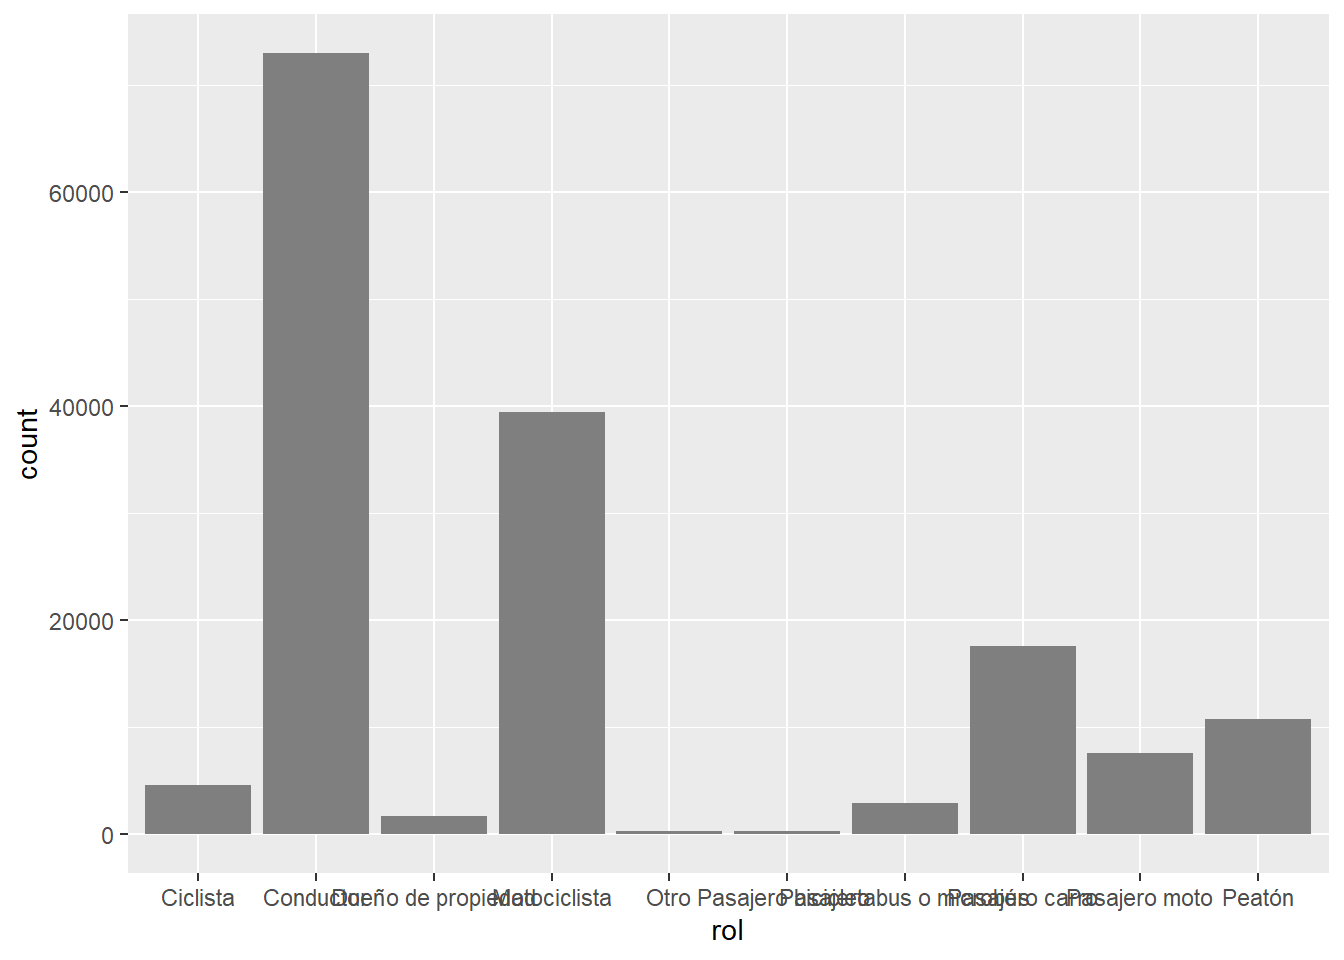
\includegraphics{Regresion_files/figure-latex/unnamed-chunk-17-1.pdf}

\textbf{Dividir Datos}

\begin{Shaded}
\begin{Highlighting}[]
\KeywordTok{set.seed}\NormalTok{(}\DecValTok{124}\NormalTok{)}

\NormalTok{y =}\StringTok{  }\NormalTok{dplyr}\OperatorTok{::}\KeywordTok{pull}\NormalTok{(autos, mpg)}

\NormalTok{autos}\OperatorTok{$}\NormalTok{dividir_datos <-}\StringTok{ }\KeywordTok{sample.split}\NormalTok{(y, }\DataTypeTok{SplitRatio=}\FloatTok{0.70}\NormalTok{)}

\NormalTok{autos_training =}\StringTok{ }\KeywordTok{subset}\NormalTok{(autos, autos}\OperatorTok{$}\NormalTok{dividir_datos}\OperatorTok{==}\OtherTok{TRUE}\NormalTok{)}
\NormalTok{autos_testing =}\StringTok{ }\KeywordTok{subset}\NormalTok{(autos, autos}\OperatorTok{$}\NormalTok{dividir_datos}\OperatorTok{==}\OtherTok{FALSE}\NormalTok{)}
\end{Highlighting}
\end{Shaded}

\textbf{Modelo Lineal}

\begin{Shaded}
\begin{Highlighting}[]
\NormalTok{linear_model =}\StringTok{ }\KeywordTok{lm}\NormalTok{(mpg }\OperatorTok{~}\StringTok{ }\NormalTok{hp }\OperatorTok{+}\StringTok{ }\NormalTok{weight, }
                  \DataTypeTok{data=}\NormalTok{autos_training)}
\end{Highlighting}
\end{Shaded}

\textbf{Evaluacion del modelo}

\begin{Shaded}
\begin{Highlighting}[]
\NormalTok{mpg_predict <-}\StringTok{ }\KeywordTok{predict}\NormalTok{(linear_model, }\DataTypeTok{newdata =}\NormalTok{ autos_testing)  }\CommentTok{# predict mpg}
\KeywordTok{mse}\NormalTok{(autos_testing}\OperatorTok{$}\NormalTok{mpg, mpg_predict)}
\end{Highlighting}
\end{Shaded}

\begin{verbatim}
## [1] 0.02530576
\end{verbatim}

\hypertarget{ejemplo-usando-la-libreria-bestnorm}{%
\paragraph{\texorpdfstring{\textbf{Ejemplo usando la libreria
BestNorm}}{Ejemplo usando la libreria BestNorm}}\label{ejemplo-usando-la-libreria-bestnorm}}

\textbf{Carga de los Datos}

\begin{Shaded}
\begin{Highlighting}[]
\NormalTok{autos <-}\StringTok{ }\KeywordTok{read_csv}\NormalTok{(}\StringTok{"auto-mpg_g.csv"}\NormalTok{)}
\end{Highlighting}
\end{Shaded}

\begin{verbatim}
## Parsed with column specification:
## cols(
##   mpg = col_double(),
##   cyl = col_double(),
##   disp = col_double(),
##   hp = col_double(),
##   weight = col_double(),
##   acc = col_double(),
##   model.year = col_double(),
##   origin = col_double(),
##   model.name = col_character()
## )
\end{verbatim}

\begin{Shaded}
\begin{Highlighting}[]
\KeywordTok{head}\NormalTok{(autos, }\DecValTok{400}\NormalTok{)}
\end{Highlighting}
\end{Shaded}

\begin{verbatim}
## # A tibble: 398 x 9
##      mpg   cyl  disp    hp weight   acc model.year origin model.name       
##    <dbl> <dbl> <dbl> <dbl>  <dbl> <dbl>      <dbl>  <dbl> <chr>            
##  1    18     8   307   130   3504    12         70      1 chevrolet chevel~
##  2    15     8   350   165   3693    12         70      1 buick skylark 320
##  3    18     8   318   150   3436    11         70      1 plymouth satelli~
##  4    16     8   304   150   3433    12         70      1 amc rebel sst    
##  5    17     8   302   140   3449    11         70      1 ford torino      
##  6    15     8   429   198   4341    10         70      1 ford galaxie 500 
##  7    14     8   454   220   4354     9         70      1 chevrolet impala 
##  8    14     8   440   215   4312     9         70      1 plymouth fury iii
##  9    14     8   455   225   4425    10         70      1 pontiac catalina 
## 10    15     8   390   190   3850     9         70      1 amc ambassador d~
## # ... with 388 more rows
\end{verbatim}

\textbf{Datos antes de normalizar vs normalizados}

\begin{Shaded}
\begin{Highlighting}[]
\KeywordTok{hist}\NormalTok{(autos}\OperatorTok{$}\NormalTok{mpg)}
\end{Highlighting}
\end{Shaded}

\includegraphics{Regresion_files/figure-latex/unnamed-chunk-22-1.pdf}

\begin{Shaded}
\begin{Highlighting}[]
\KeywordTok{hist}\NormalTok{(autos}\OperatorTok{$}\NormalTok{weight)}
\end{Highlighting}
\end{Shaded}

\includegraphics{Regresion_files/figure-latex/unnamed-chunk-22-2.pdf}

\begin{Shaded}
\begin{Highlighting}[]
\KeywordTok{hist}\NormalTok{(autos}\OperatorTok{$}\NormalTok{disp)}
\end{Highlighting}
\end{Shaded}

\includegraphics{Regresion_files/figure-latex/unnamed-chunk-22-3.pdf}

\begin{Shaded}
\begin{Highlighting}[]
\KeywordTok{hist}\NormalTok{(}\KeywordTok{orderNorm}\NormalTok{(autos}\OperatorTok{$}\NormalTok{mpg)}\OperatorTok{$}\NormalTok{x.t, }\DataTypeTok{col=}\StringTok{"#cfbae1"}\NormalTok{,}\DataTypeTok{border=}\StringTok{"#c59fc9"}\NormalTok{)}
\end{Highlighting}
\end{Shaded}

\includegraphics{Regresion_files/figure-latex/unnamed-chunk-22-4.pdf}

\begin{Shaded}
\begin{Highlighting}[]
\KeywordTok{hist}\NormalTok{(}\KeywordTok{orderNorm}\NormalTok{(autos}\OperatorTok{$}\NormalTok{weight)}\OperatorTok{$}\NormalTok{x.t, }\DataTypeTok{col=}\StringTok{"#cfbae1"}\NormalTok{,}\DataTypeTok{border=}\StringTok{"#c59fc9"}\NormalTok{)}
\end{Highlighting}
\end{Shaded}

\includegraphics{Regresion_files/figure-latex/unnamed-chunk-22-5.pdf}

\begin{Shaded}
\begin{Highlighting}[]
\KeywordTok{hist}\NormalTok{(}\KeywordTok{orderNorm}\NormalTok{(autos}\OperatorTok{$}\NormalTok{disp)}\OperatorTok{$}\NormalTok{x.t, }\DataTypeTok{col=}\StringTok{"#cfbae1"}\NormalTok{,}\DataTypeTok{border=}\StringTok{"#c59fc9"}\NormalTok{)}
\end{Highlighting}
\end{Shaded}

\includegraphics{Regresion_files/figure-latex/unnamed-chunk-22-6.pdf}

\textbf{Preparacion de los datos:}

\begin{Shaded}
\begin{Highlighting}[]
\CommentTok{# Ya que tenemos valores en 0 dentro de la variable caballos de fuerza, necesitamos excluir esos datos para no afectar nuestros calculos.}
\NormalTok{autos <-}\StringTok{ }\NormalTok{autos[}\OperatorTok{!}\NormalTok{(autos}\OperatorTok{$}\NormalTok{hp }\OperatorTok{==}\StringTok{ }\DecValTok{0}\NormalTok{),]}

\CommentTok{# Llenar los valores nulos en la columna caballos de fuerza}
\NormalTok{media_hp =}\StringTok{ }\KeywordTok{median}\NormalTok{(autos}\OperatorTok{$}\NormalTok{hp)}
\NormalTok{autos}\OperatorTok{$}\NormalTok{hp[}\KeywordTok{is.na}\NormalTok{(autos}\OperatorTok{$}\NormalTok{hp)] <-}\StringTok{ }\NormalTok{media_hp}

\CommentTok{# Dividir los valores de la columna modelo para extraer solo el fabricante, ya que al tener 305 modelos estabamos perdiendo variabilidad en los datos}
\NormalTok{autos <-}\StringTok{ }\NormalTok{autos }\OperatorTok\StringTok{ }\KeywordTok{separate}\NormalTok{(model.name, }
                \KeywordTok{c}\NormalTok{(}\StringTok{"manufacturer"}\NormalTok{))}

\CommentTok{# Normalizar las variables que vamos a usar}
\NormalTok{mpg_normalized <-}\StringTok{ }\KeywordTok{orderNorm}\NormalTok{(autos}\OperatorTok{$}\NormalTok{mpg)}\OperatorTok{$}\NormalTok{x.t}
\NormalTok{weight_normalized <-}\StringTok{ }\KeywordTok{orderNorm}\NormalTok{(autos}\OperatorTok{$}\NormalTok{weight)}\OperatorTok{$}\NormalTok{x.t}
\NormalTok{disp_normalized <-}\StringTok{ }\KeywordTok{orderNorm}\NormalTok{(autos}\OperatorTok{$}\NormalTok{disp)}\OperatorTok{$}\NormalTok{x.t}
\NormalTok{hp_normalized <-}\StringTok{ }\KeywordTok{orderNorm}\NormalTok{(autos}\OperatorTok{$}\NormalTok{hp)}\OperatorTok{$}\NormalTok{x.t}

\NormalTok{autos}\OperatorTok{$}\NormalTok{mpg <-}\StringTok{ }\NormalTok{mpg_normalized}
\NormalTok{autos}\OperatorTok{$}\NormalTok{weight <-}\StringTok{ }\NormalTok{weight_normalized}
\NormalTok{autos}\OperatorTok{$}\NormalTok{disp <-}\StringTok{ }\NormalTok{disp_normalized}
\NormalTok{autos}\OperatorTok{$}\NormalTok{hp <-}\StringTok{ }\NormalTok{hp_normalized}
\KeywordTok{head}\NormalTok{(autos, }\DecValTok{400}\NormalTok{)}
\end{Highlighting}
\end{Shaded}

\begin{verbatim}
## # A tibble: 392 x 9
##       mpg   cyl  disp    hp weight   acc model.year origin manufacturer
##     <dbl> <dbl> <dbl> <dbl>  <dbl> <dbl>      <dbl>  <dbl> <chr>       
##  1 -0.561     8 0.870 0.705  0.587    12         70      1 chevrolet   
##  2 -1.02      8 1.18  1.33   0.738    12         70      1 buick       
##  3 -0.561     8 0.967 1.06   0.542    11         70      1 plymouth    
##  4 -0.843     8 0.789 1.06   0.535    12         70      1 amc         
##  5 -0.713     8 0.713 0.816  0.564    11         70      1 ford        
##  6 -1.02      8 2.02  1.84   1.35     10         70      1 ford        
##  7 -1.24      8 2.28  2.20   1.37      9         70      1 chevrolet   
##  8 -1.24      8 2.16  2.07   1.31      9         70      1 plymouth    
##  9 -1.24      8 2.49  2.37   1.52     10         70      1 pontiac     
## 10 -1.02      8 1.56  1.73   0.861     9         70      1 amc         
## # ... with 382 more rows
\end{verbatim}

\textbf{Correlaciones}

\begin{Shaded}
\begin{Highlighting}[]
\KeywordTok{ggpairs}\NormalTok{(autos,}\DataTypeTok{columns =} \KeywordTok{c}\NormalTok{(}\DecValTok{1}\NormalTok{, }\DecValTok{3}\NormalTok{, }\DecValTok{4}\NormalTok{, }\DecValTok{5}\NormalTok{, }\DecValTok{6}\NormalTok{, }\DecValTok{7}\NormalTok{))}
\end{Highlighting}
\end{Shaded}

\includegraphics{Regresion_files/figure-latex/unnamed-chunk-24-1.pdf}

\textbf{Dividir Datos}

\begin{Shaded}
\begin{Highlighting}[]
\KeywordTok{set.seed}\NormalTok{(}\DecValTok{124}\NormalTok{)}

\NormalTok{y =}\StringTok{  }\NormalTok{dplyr}\OperatorTok{::}\KeywordTok{pull}\NormalTok{(autos, mpg)}

\NormalTok{autos}\OperatorTok{$}\NormalTok{dividir_datos <-}\StringTok{ }\KeywordTok{sample.split}\NormalTok{(y, }\DataTypeTok{SplitRatio=}\FloatTok{0.70}\NormalTok{)}

\NormalTok{autos_training =}\StringTok{ }\KeywordTok{subset}\NormalTok{(autos, autos}\OperatorTok{$}\NormalTok{dividir_datos}\OperatorTok{==}\OtherTok{TRUE}\NormalTok{)}
\NormalTok{autos_testing =}\StringTok{ }\KeywordTok{subset}\NormalTok{(autos, autos}\OperatorTok{$}\NormalTok{dividir_datos}\OperatorTok{==}\OtherTok{FALSE}\NormalTok{)}
\end{Highlighting}
\end{Shaded}

\textbf{Modelo Lineal}

\begin{Shaded}
\begin{Highlighting}[]
\NormalTok{linear_model =}\StringTok{ }\KeywordTok{lm}\NormalTok{(mpg }\OperatorTok{~}\StringTok{ }\NormalTok{hp }\OperatorTok{+}\StringTok{ }\NormalTok{weight, }
                  \DataTypeTok{data=}\NormalTok{autos_training)}
\end{Highlighting}
\end{Shaded}

\textbf{Evaluacion del modelo}

\begin{Shaded}
\begin{Highlighting}[]
\NormalTok{mpg_predict <-}\StringTok{ }\KeywordTok{predict}\NormalTok{(linear_model, }\DataTypeTok{newdata =}\NormalTok{ autos_testing)  }\CommentTok{# predict mpg}
\KeywordTok{mse}\NormalTok{(autos_testing}\OperatorTok{$}\NormalTok{mpg, mpg_predict)}
\end{Highlighting}
\end{Shaded}

\begin{verbatim}
## [1] 0.2542667
\end{verbatim}


\end{document}
